\documentclass[../../main.tex]{subfiles}

\begin{document}

\defaultchapter{Sequences and Series}

\section{What is a sequence?}

A \textbf{sequence} is essentially a ordered list of ``elements", usually numbers.
\[
    \underbrace{1}_\text{\nth{1} element},\quad
    \underbrace{2}_\text{\nth{2} element},\quad
    \underbrace{4}_\text{\nth{3} element},\quad
    \underbrace{8}_\text{\nth{4} element},\quad
    \underbrace{16}_\text{\nth{5} element},\quad
    \ldots
\]

\noindent Suppose the above sequence is called \(u\). Any specific element is identified by its \textbf{index}:
\begin{align}
    u_1 &= 1 \indent (\text{\nth{1} element})\\
    u_2 &= 2 \indent (\text{\nth{2} element})\\
    u_3 &= 4 \indent (\text{\nth{3} element})\\
    \vdots
\end{align}

There are many ways to define a sequence. One way is with an explicit formula in terms of its index, \(n\):
\[
    u_n = 2^{n-1}
\]
where we can plug in values and get back the \(n\)\textsuperscript{th} element of the sequence. Though the value of \(n\) can be anything, it is usually restricted to positive integers (1, 2, 3, \ldots), so the example above has the same elements as the sequence shown previously.

\begin{insight}{~}
We can think of sequences as a function \(u\) that maps from non-negative integers to the elements of the sequence, defined with an expression
\[
    u(n) = 2^{n-1}, n\in\{0, 1, 2, \ldots\}
\]
or defined with the domain/range explicitly
\[
    u: \begin{cases}
    1\to1\\
    2\to2\\
    3\to4\\
    \vdots
    \end{cases}
\]
for finite sequences. However, it is convention to write the function's argument as a subscript ($ u_n$ instead of $u(n)$).
\end{insight}

\subsection{Recursive sequences}

Another way of defining sequences is using what is known as a \textbf{recursive definition}. This definition also uses a formula, but that formula refers back to previous terms of the sequence. For example,
\[
    u_n = 2\cdot u_{n-1}.
\]
However, this formula by itself is incomplete. We need to provide some initial term(s) with the recursive formula in order to define the sequence. We must add an initial term, such as
\[
    u_1 = 1,\quad u_n = 2\cdot u_{n-1}.
\]
Notice how this is the same sequence as the one introduced at the beginning of this chapter (plug it in and check!). Not only are these different ways of \emph{defining} a sequence, they are also different ways of \emph{representing} sequences. Crucially, sequences can be expressed in more than one way (e.g. with an explicit formula, a recursive formula, etc).

One of the most famous sequences defined in this way is the Fibonacci sequence. It starts with \(F_1 = 1\) and \(F_2 = 1\), every following term being the sum of the last two terms. Mathematically, this is written as
\[
    F_1 = 1,\quad F_2 = 1,\quad F_n = F_{n-1} + F_{n-2}
\]
which gives rise to the Fibonacci numbers.
\[
    1, 1, 2, 3, 5, 8, 13, 21, 34, 55, \ldots
\]

\section{What is a series?}

A series is the sum of the terms in a sequence (basically replace the commas with plus signs). For example,
\[
    1+2+4+8+16+\ldots
\]
Given a sequence \( u_n\), the sum of the first \(n\) terms is denoted by \(S_n\).
\begin{align}
    S_1 &= u_1\\
    S_2 &= u_1 + u_2\\
    S_3 &= u_1 + u_2 + u_3\\
    S_n &= u_1 + u_2 + \ldots + u_{n-1} + u_n
\end{align}

Repeated summation can often get long and cluttered to write out fully, so a more concise notation was introduced: \textbf{Sigma notation}, using the Greek letter \(\Sigma\).
\[
    \sum_{i=0}^6i^2 = 0^2 + 1^2 + 2^2 + 3^2 + 4^2 + 5^2 + 6^2
\]
The variable goes through the integers from the bottom number to the top number (inclusive, in the example \(i\) from 0 to 6), the lower and upper bounds, and all these terms are summed. Of course, the upper bound must be larger than the lower bound. An infinite sum can also be represented using Sigma notation by making the upper bound infinity:
\[
    \sum_{n=1}^{\infty}n = 1 + 2 + 3 + 4 + \ldots
\]
However, infinite sums are not always \emph{defined}. For example, the infinite sum above doesn't have a definite value since it gets larger and larger (in other words, it doesn't \emph{converge} to anything). If the sum \emph{approaches} a specific value, we can say it equals that value. (More on limits and convergence in later chapters.)

\begin{extension}{Basel Problem}
A famous example of a converging infinite series is the following:
\[
    \sum_{n=1}^{\infty}\frac1{n^2} = 1 + \frac14 + \frac19 + \frac1{16} + \ldots
\]
Finding the exact value of this particular infinite series is called the \emph{Basel problem}, and it solved by Leonhard Euler in 1735. Interestingly, the solution is:
\[
    \sum_{n=1}^{\infty}\frac1{n^2} = 1 + \frac12 + \frac19 + \frac1{16} + \ldots = \frac{\pi^2}{6}
\]
If we find the sum up till the $n$th term (called partial sums) and plot its value, it goes closer and closer to the value of $\frac{\pi^2}6$.\\
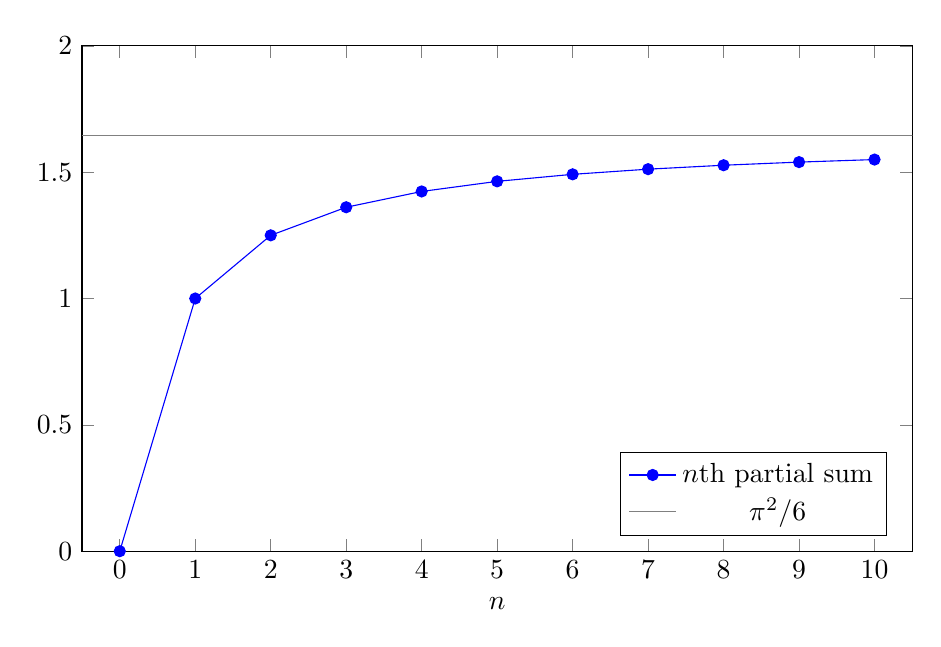
\begin{tikzpicture}
\begin{axis}[height = 8cm, width = \textwidth, xmin = -0.5, xmax = 10.5, ymin = 0, ymax = 2, legend pos=south east, xlabel = $n$]

\addplot[color = blue, mark = *]
    coordinates {
        (0,0)(1,1)(2,1.25)(3,1.3611)(4,1.4236)(5,1.4636)(6,1.4914)(7,1.5118)(8,1.5274)(9,1.5398)(10,1.5498)
    };
    \addlegendentry{$n$th partial sum}
\addplot[color = gray, domain = -1:11]
    {1.6449};
    \addlegendentry{\(\pi^2/6\)}
\end{axis}
\end{tikzpicture}
\end{extension}

Using this, we can write the expression for \(S_n\) like so:
\[
    S_n = u_1 + u_2 + \ldots + u_{n-1} + u_n = \sum_{i=1}^n u_i
\]

Certain groups of sequences/series have nice properties and patterns, so mathematicians classify them based on their characteristics. This syllabus will focus on two such classes of sequences and series: \textbf{arithmetic} and \textbf{geometric} sequences and series.

\section{Arithmetic Sequences}

Arithmetic sequences have consecutive elements separated by a constant value, aptly named the sequence's \textbf{common difference}.
\[
    1\underbrace{,\quad}_{+3}
    4\underbrace{,\quad}_{+3}
    7\underbrace{,\quad}_{+3}
    10\underbrace{,\quad}_{+3}
    13\underbrace{,\quad}_{+3}
    \ldots
\]
\begin{tikzpicture}
\begin{axis}[height = 12cm, width = \textwidth, ytick = {0,5,10,15,20,25,30}, xlabel = {\(n\)}, ylabel = {\(u_n\)}, legend pos=south east]

\addplot[color = blue, mark = *, samples = 10, domain = 1:10]
    {3*x - 2};
    \addlegendentry{1, 4, 7, \ldots}

\end{axis}
\end{tikzpicture}

When plotted on a set of axes, the elements create a straight line (the slope of which is the common difference). To find the common difference of an arithmetic sequence, we can take any element and subtract the previous element.
\[
    u_n - u_{n-1} = d
\]

\begin{theorem}{Arithmetic Sequence (General Formula)}
Any general arithmetic sequence with a common difference \(d\) would have the elements
\[
    u_1,\quad u_1+d,\quad u_1+2d,\quad u_1+3d,\quad u_1+4d,\quad \ldots
\]
This gives rise to the general formula for an arithmetic sequence. (Plug values for \(n\) in to see if it matches the above sequence!)
\formula{u_n = u_1 + (n-1)d}{SL 1.2.1}
\end{theorem}

\begin{example}{Arithmetic Sequence}
Find the general formula for the arithmetic sequence:
\[
    1, 4, 7, 10, 13, \ldots
\]

\sep
The general formula requires the first element and common difference. The first element is \(u_1 = 1\), and the common difference can be found using any two consecutive elements, so using the first two gives \(d = u_2 - u_1 = 4 - 1 = 3\).
\begin{align}
    u_n &= u_1 + (n-1)d\\
    &= 1 + (n-1)\cdot3\\
    &= 3n - 2
\end{align}
\end{example}

\subsection{Arithmetic Series}

Suppose we want to find \(S_6\) of the sequence shown in the previous example. We could add up all the terms individually,
\[
    S_6=1+4+7+10+13+16
\]
but an easier way to calculate it is by noticing that elements on opposite ends add to the same value. We could pair each term like this:
\begin{align}
    S_6&=1+4+7+10+13+16\\
    +S_6&=16+13+10+7+4+1\\
    2S_6&=17+17+17+17+17+17
\end{align}
We can now express the sum as adding the same number over and over again, which is the same as multiplication!
\begin{align}
    2S_6 = 17+17+17+17+17+17 &= 6\times17\\
    S_6 &= 3\times17 = 51
\end{align}
This idea of pairing up terms on opposite ends of the series generalizes nicely, and we can use it to find a general formula for \(S_n\) for \emph{any} arithmetic series!

Lets start with a general arithmetic series:
\[
    S_n = \underbrace{u_1 + u_2 + \ldots + u_{n-1} + u_n}_{n\text{ terms}}
\]
We can write everything in terms of \(u_1\) and the common difference \(d\).
\[
    S_n = \underbrace{(u_1) + (u_1 + d) + \ldots + (u_1 + (n-2)d) + (u_1 + (n-1)d)}_{n\text{ terms}}
\]
From here, we can use the same trick of pairing terms from earlier.
\begin{align}
    S_n &= (u_1) &+& (u_1 + d) &+ \ldots\\
    +S_n &= (u_1 + (n-1)d) &+& (u_1 + (n-2)d) &+ \ldots\\
    2S_n &= (u_1 + u_1 + (n-1)d) &+& (u_1 + d + u_1 + (n-2)d) &+ \ldots\\
    &= (2u_1 + (n-1)d) &+& (2u_1 + (n-1)d) &+ \ldots
\end{align}
Again, all the terms here are the same, and repeated addition is simply multiplication!
\[
    2S_n = \underbrace{(2u_1 + (n-1)d) + (2u_1 + (n-1)d) + \ldots}_{n\text{ terms}} = n(2u_1 + (n-1)d)
\]

{\hfill\Large\bfseries NEEDS FIXING\hfill}
\begin{lstlisting}
\begin{formula}
\formula{S_n = \frac{n}2(2u_1+(n-1)d)}{SL 1.2.2}
\end{formula}
 \end{lstlisting}

\begin{thinking}{~}
    If we're only adding integers, we know our total sum must be an integer. However, the sum formula contains a division by 2\ldots How can we be sure that the division by 2 does not cause the formula to spit out non-integer values?
\end{thinking}

Since we know that pairing opposite end terms of an arithmetic series yields equal terms, we can translate this into an equivalent formula for \(S_n\).

{\hfill\Large\bfseries NEEDS FIXING\hfill}
\begin{lstlisting}
\begin{formula}
    S_n = \frac{n}2(u_1 + u_n)
\end{formula}
 \end{lstlisting}

\begin{example}{Arithmetic Series 1}
Find the general formula for the arithmetic series
\[
    1 + 4 + 7 + 10 + 13 + \ldots
\]

\sep
We found previously the first term \(a_1 = 1\) and common difference \(d = 3\) for this sequence, so we can simply plug them into the formula.
\[
    S_n = \frac{n}2(2u_1+(n-1)d) = \frac{n}2(2(1)+(n-1)\cdot3) = \frac{3n^2-n}2
\]
(Plug in values to check that this formula does indeed work!)
\end{example}

\begin{thinking}{~}
The general sum formula \(S_n\) for most arithmetic series would be a quadratic expression, meaning it has a \(n^2\) term, like the one in the example above. Can you think of the case(s) where the general sum formula of an arithmetic series is \emph{not} a quadratic expression?
\end{thinking}

Since each next \(n\) adds on one more term to \(S_n\), we can find a way of getting the original sequence back from the series,
\[
    S_1 = u_1,\quad S_2 - S_1 = u_2,\quad S_3 - S_2 = u_3,\quad \ldots
\]
or in general,
\[
    S_n - S_{n - 1} = u_n.
\]

\begin{example}{Arithmetic Series 2}
Find the sequence with the corresponding series formula
\[
    S_n = 8n - 2n^2
\]
\sep
We know that \(S_1 = u_1\), so
\[
    S_1 = 8(1) - 2(1)^2 = 6 = u_1.
\]
Now we need one more equation to find \(d\). We can use any value of \(n\), but I will use \(n = 2\) here for simplicity.
\begin{align}
    S_2 = \frac{2}2(2a_1 + ((2)-1)d) = 2u_1 + d = 2(6) + d &= 12 + d\\
    S_2 = 8(2) - 2(2)^2 &= 8\\
    12 + d &= 8 \implies d = -4
\end{align}
\end{example}

\begin{questions}{Drills}
Find the common difference of these arithmetic sequences:
\begin{question_set}(3)
    \item -66, -81, -96, \ldots
    \item -301, -275, -249, \ldots
    \item 345, 353, 361, \ldots
    \item -23, 0, 23, \ldots
    \item 128, 113, 98, \ldots
    \item -395, -376, -357, \ldots
\end{question_set}

Find the \nth{18} element of these arithmetic sequences:
\begin{question_set}(3)
    \item 47, 64, 81, \ldots
    \item -141, -156, -171, \ldots
    \item 7, -11, -29, \ldots
    \item 20, 12, 4, \ldots
    \item 7, 11, 15, \ldots
    \item -81, -84, -87, \ldots
\end{question_set}

Find the sum of the first 13 elements of these arithmetic sequences:
\begin{question_set}(3)
    \item -28, -40, -52, \ldots
    \item -53, -61, -69, \ldots
    \item -49, -54, -59, \ldots
    \item 6, 7, 8, \ldots
    \item 1, -9, -19, \ldots
    \item -27, -29, -31, \ldots
\end{question_set}

Find the formula for the arithmetic sequence given its general sum formula:
\begin{question_set}(2)
    \item \(S_n=-5.5n^2 + -12.5n\)
    \item \(S_n=13.5n^2 + 185.5n\)
    \item \(S_n=-3.5n^2 + 43.5n\)
    \item \(S_n=6n^2 + 23.5n\)
    \item \(S_n=10.75n^2 + 25.25n\)
    \item \(S_n=7n^2 + 61.5n\)
    \item \(S_n=-7n^2 + 91n\)
    \item \(S_n=-10n^2 + -201n\)
\end{question_set}
\end{questions}

\section{Geometric Sequences}

Geometric sequences have consecutive elements share a constant ratio, aptly named the sequence's \textbf{common ratio}.
\[
    1\underbrace{,\quad}_{\times3}
    3\underbrace{,\quad}_{\times3}
    9\underbrace{,\quad}_{\times3}
    27\underbrace{,\quad}_{\times3}
    81\underbrace{,\quad}_{\times3}
    \ldots
\]
To find the common ratio of a geometric sequence, we can take any element and divide the previous element:
\[
    \frac{u_{n+1}}{u_n} = r
\]

\begin{center}
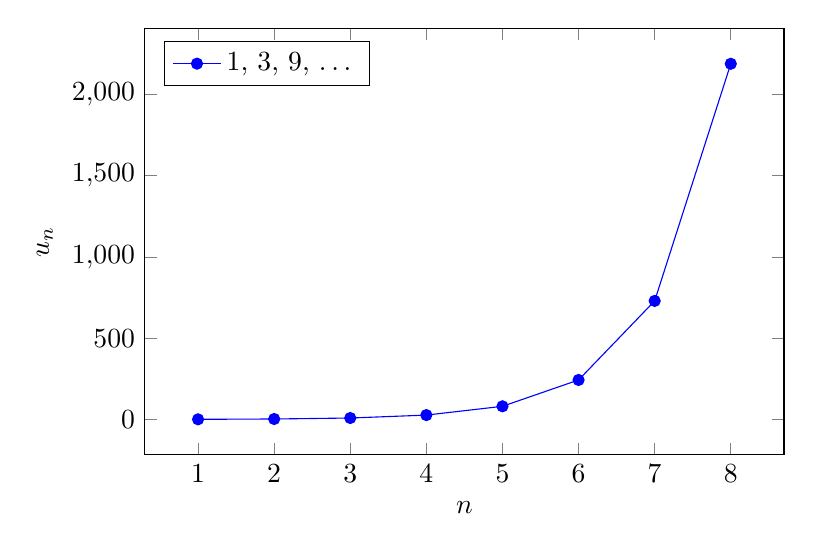
\begin{tikzpicture}
\begin{axis}[height = 7cm, width = 0.8\textwidth, xlabel = {\(n\)}, ylabel = {\(u_n\)}, xtick = {1, 2, 3, 4, 5, 6, 7, 8}, legend pos=north west]

\addplot[color = blue, mark = *, samples = 8, domain = 1:8]
    {3^(x - 1)};
    \addlegendentry{1, 3, 9, \ldots}

\end{axis}
\end{tikzpicture}
\end{center}

\begin{wrapfigure}{R}{0.51\textwidth}
    \centering
    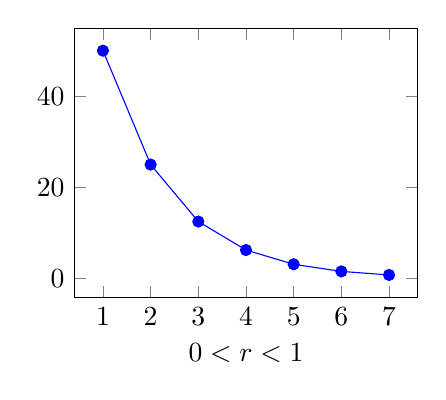
\begin{tikzpicture}
\begin{axis}[height = 5cm, width = 0.49\textwidth, xtick = {1, 2, 3, 4, 5, 6, 7}, xlabel = \(0 < r < 1\)]

\addplot[color = blue, mark = *, samples = 7, domain = 1:7]
    {100*(0.5)^x};

\end{axis}
    \end{tikzpicture}
\end{wrapfigure}

Plotting the above elements on a set of axes creates an exponential curve. This example behaves this way because \(r > 1\). There are 3 other ways in which geometric sequences can behave, examples of which are shown in the graphs. Generally, geometric sequences tend to grow or shrink exponentially depending on the absolute value of $r$, and alternate between positive and negative elements based on whether $r$ is positive or negative.

\begin{figure}[h]
    \centering
    \begin{subfigure}{0.49\textwidth}
        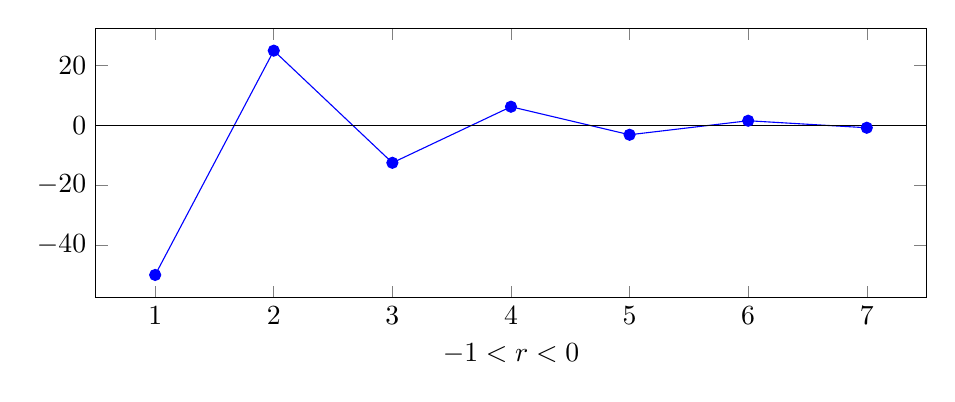
\begin{tikzpicture}
            \begin{axis}[height = 5cm, width = \textwidth, xmin = 0.5, xmax = 7.5, xtick = {1, 2, 3, 4, 5, 6, 7}, xlabel = \(-1 < r < 0\)]

                \addplot[color = blue, mark = *, samples = 7, domain = 1:7]
                {100*(-0.5)^x};
    
                \addplot[color = black, domain = 0:8, thin]
                    {0};

            \end{axis}
        \end{tikzpicture}
    \end{subfigure}
    \begin{subfigure}{0.49\textwidth}
        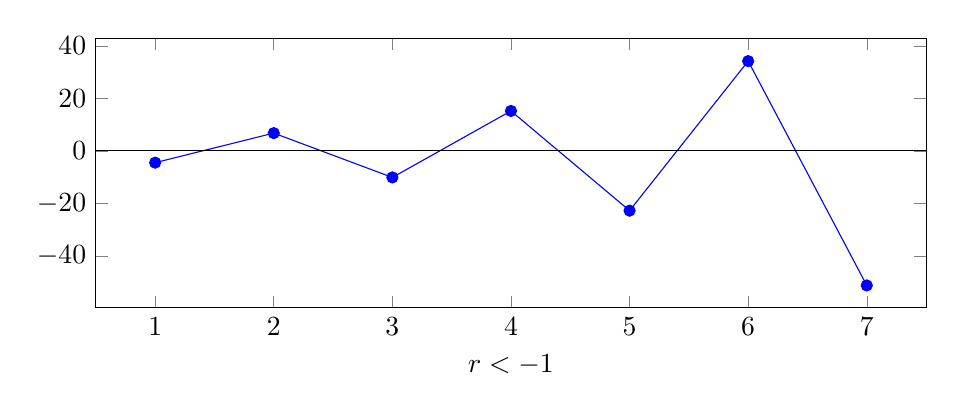
\begin{tikzpicture}
            \begin{axis}[height = 5cm, width = \textwidth, xmin = 0.5, xmax = 7.5, xtick = {1, 2, 3, 4, 5, 6, 7}, xlabel = \(r < -1\)]
            
                \addplot[color = blue, mark = *, samples = 7, domain = 1:7]
                {3*(-1.5)^x};
                
                \addplot[color = black, domain = 0:8, thin]
                {0};

            \end{axis}
        \end{tikzpicture}
    \end{subfigure}
\end{figure}

\begin{thinking}{Edge Cases}
    What is the behaviour of geometric sequences when the common ratio is between the ranges shown below the graphs? (namely, the cases \(r = 1\), \(r = 0\), and \(r = -1\))
\end{thinking}

Any general geometric sequence with a common ratio \(r\) has the elements
\[
    u_1,\quad u_1r,\quad u_1r^2,\quad u_1r^3,\quad u_1r^4,\quad \ldots
\]
This gives rise to the general formula for a geometric sequence, which is in the formula booklet. (Plug values for \(n\) in to see if it matches the above sequence!).

\formula{u_n = u_1r^{n - 1}}{}

\begin{example}{Geometric Sequence}
Find the general formula for the geometric sequence:
\[
    1, 3, 9, 27, 81, \ldots
\]
\sep
The general formula requires the first element and common ratio. The first element is \(u_1 = 1\), and the common ratio can be found using any two consecutive elements, so using the first two gives \(r = \frac{u_2}{u_1} = \frac31 = 3\).
\[
    u_n = u_1r^{n-1} = 1(3)^{n-1} = 3^{n-1}
\]
\end{example}

\subsection{Geometric Series}

The derivation of the general formula for geometric series is outside the scope of this chapter, nevertheless, this formula works the same way as the other sum formula - we plug in values for \(u_1\) and \(r\) to get an expression in terms of n.

{\hfill\Large\bfseries NEEDS FIXING\hfill}
\begin{lstlisting}
\begin{formula}
    S_n = \frac{u_1(r^n - 1)}{r - 1} = \frac{u_1(1 - r^n)}{1 - r},\quad r\neq1
\end{formula}
 \end{lstlisting}

Similar to before, the same property holds for consecutive \(S_n\) terms:
\[
    S_n - S_{n - 1} = u_n
\]

\begin{example}{Geometric Series}
Find the general formula for the geometric series
\[
    1 + 3 + 9 + 27 + 81 + \ldots
\]
\sep
We found previously the first term \(u_1 = 1\) and common ratio \(r = 3\) for this sequence, so we can simply plug them into the formula.
\[
    S_n = u_1\frac{1 - r^n}{1 - r} = (1)\frac{1 - (3)^n}{1 - (3)} = \frac{3^n - 1}2
\]
\end{example}

\subsection{Infinite Geometric Series}

If the common ratio is between -1 and 1, then the elements of the sequence tend to get smaller and smaller.
\[
    u_1 = 1, r = \frac12 \implies 1 + \frac12 + \frac14 + \frac18 + \frac1{16} + \ldots
\]
\begin{center}
\begin{tikzpicture}
\begin{axis}[height = 8cm, width = 0.8\textwidth, xlabel = {\(n\)}, ylabel = {\(S_n\)}, xmin = 0.5, xmax = 11.5, legend pos=south east]

\addplot[draw = none, color = blue, mark = *, samples = 11, domain = 1:11]
    {2 - 0.5^(x-1)};
    \addlegendentry{\(S_n\)};

\addplot[color = gray, domain = -1:11]
    {2};
    \addlegendentry{\(2\)};
\end{axis}
\end{tikzpicture}
\end{center}

For all such geometric series, the sum does approach a specific value as more and more terms are added. This is called an \textbf{infinite sum}, denoted by \(S_\infty\), and is only defined for geometric series with \(|r|<1\). As \(n\) gets larger and larger, the \(r^n\) in the sum formula tends towards 0, giving the exact value the sum converges onto (more about \emph{limits} and \emph{convergence} in later chapters).

{\hfill\Large\bfseries NEEDS FIXING\hfill}
\begin{lstlisting}
\begin{formula}
    S_\infty = \frac{u_1}{1-r},\quad|r|<1
\end{formula}
 \end{lstlisting}

\begin{example}{Infinite Geometric Series}
Find the sum to infinity for the following series:
\[
    8 - 2 + \frac12 - \frac18 + \frac1{32} - \ldots
\]

\sep
The first term is \(u_1 = 8\), and the common ratio can be found using the first two terms \(\frac{-2}8 = -\frac14\). Since \(|r|<1\), the infinite sum will be defined. Plugging these values into the formula yields
\[
    S_\infty = \frac{(8)}{1-(-\frac14)} = \frac{32}{5}
\]
(Try adding the sum's terms on a calculator to see that it does approach $\frac{32}{5}$!)
\end{example}

\begin{questions}{Drills}
Find the common ratio of these geometric sequences:
\begin{question_set}(3)
    \item 784, -112, 16, \ldots
    \item -256, -64, -16, \ldots
    \item -18, -90, -450, \ldots
    \item -432, -144, -48, \ldots
    \item 486, 162, 54, \ldots
    \item -47, 188, -752, \ldots
\end{question_set}

Find the \nth{8} element of these geometric sequences:
\begin{question_set}(3)
    \item 17, -17, 17, \ldots
    \item -180, 60, -20, \ldots
    \item -20, -40, -80, \ldots
    \item 720, 180, 45, \ldots
    \item 60, 120, 240, \ldots
    \item 54, 216, 864, \ldots
\end{question_set}

Find the sum of the first 12 terms of these geometric sequences:
\begin{question_set}(3)
    \item -21, 63, -189, \ldots
    \item -180, -60, -20, \ldots
    \item -23, 92, -368, \ldots
    \item -52, 312, -1872, \ldots
    \item -5100, -510, -51, \ldots
    \item -192, -96, -48, \ldots
\end{question_set}

Find the sum to infinity for the following infinite geometric series:
\begin{question_set}(3)
    % \item 47, -11.75, 2.9375, \ldots
    \item 51, 10.2, 2.04, \ldots
    % \item 91, -18.2, 3.64, \ldots
    \item 93, -18.6, 3.72, \ldots
    \item 34, -17, 8.5, \ldots
    \item 41, 20.5, 10.25, \ldots
    \item 99, -33, 11, \ldots
    \item 39, -7.8, 1.56, \ldots
\end{question_set}
\end{questions}

\section{Other Sequences}

Though other sequences are not a focus of the syllabus, it is good to know about \textbf{triangular numbers}. This is the sequence that counts objects arranged into triangles.
\begin{figure}[h]
    \centering
    \begin{subfigure}[h]{0.24\textwidth}
        \centering
        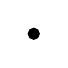
\begin{tikzpicture}
\filldraw (0, 0) circle (2pt);
        \end{tikzpicture}
        \caption*{\(t_1 = 1\)}
    \end{subfigure}
    \begin{subfigure}[h]{0.24\textwidth}
        \centering
        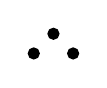
\begin{tikzpicture}
\filldraw (0, 0) circle (2pt);
\filldraw (0.5, 0) circle (2pt);
\filldraw (0.25, 0.25) circle (2pt);
        \end{tikzpicture}
        \caption*{\(t_2 = 3\)}
    \end{subfigure}
    \begin{subfigure}[h]{0.24\textwidth}
        \centering
        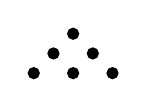
\begin{tikzpicture}
\filldraw (0, 0) circle (2pt);
\filldraw (0.5, 0) circle (2pt);
\filldraw (0.25, 0.25) circle (2pt);
\filldraw (1, 0) circle (2pt);
\filldraw (0.5, 0.5) circle (2pt);
\filldraw (0.75, 0.25) circle (2pt);
        \end{tikzpicture}
        \caption*{\(t_3 = 6\)}
    \end{subfigure}
    \begin{subfigure}[h]{0.24\textwidth}
        \centering
        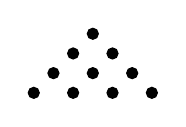
\begin{tikzpicture}
\filldraw (0, 0) circle (2pt);
\filldraw (0.5, 0) circle (2pt);
\filldraw (0.25, 0.25) circle (2pt);
\filldraw (1, 0) circle (2pt);
\filldraw (0.5, 0.5) circle (2pt);
\filldraw (0.75, 0.25) circle (2pt);
\filldraw (1.5, 0) circle (2pt);
\filldraw (1.25, 0.25) circle (2pt);
\filldraw (0.75, 0.75) circle (2pt);
\filldraw (1, 0.5) circle (2pt);
        \end{tikzpicture}
        \caption*{\(t_4 = 10\)}
    \end{subfigure}
\end{figure}

This sequence also corresponds with the sums of natural numbers.
\[
    t_n = 1 + 2 + 3 + \ldots + n
\]
This means we can apply our knowledge about arithmetic series,
\[
    t_n = \frac{n}2(u_1 + u_n) = \frac{n(1 + n)}2 = \frac{n^2 + n}2
\]
This gives us a \emph{quadratic} formula - one that has an \(n^2\) term in it. The next chapter will be all about quadratics!

\begin{summary}{Sequences and Series}
    There are many different types of sequences (arithmetic, geometric, triangular, Fibonacci) and sequence definitions (explicit, recursive). A series is the sum of elements in a sequence.

    \subtitle{Arithmetic Sequences/Series}
    Arithmetic sequences are defined by their first element and common difference.
    \[
        u_n = u_1 + (n-1)d
    \]\[
        S_n = \frac{n}2(2u_1+(n-1)d)
    \]\[
        S_n = \frac{n}2(u_1 + u_n)
    \]
    
    \subtitle{Geometric Sequences/Series}
    Geometric sequences are defined by their first element and common ratio.
    \[
        u_n = u_1r^{n - 1}
    \]\[
        S_n = u_1\frac{1 - r^n}{1 - r},\quad r\neq1
    \]\[
        S_\infty = \frac{u_1}{1-r},\quad|r|<1
    \]
\end{summary}

\end{document}